As this project is focused on the resource management framework, I will
not give a detailed description of the Hadoop Distributed File
System. Yet, I will go through some basic concepts that will make the
reader understand better the overall architecture of Hadoop.

HDFS is the distributed file system of Hadoop platform. It is designed
with the assumption that hardware failure is the norm and not an
exception making it highly fault-tolerant. Also, it is designed to run
on commodity, heterogenous, low-cost hardware making the setup and provisioning of
a cluster cheaper than HPC. HDFS has two main entities, the NameNode
(NN) and the DataNode (DN) and the architecture is depicted in Figure
\ref{fig:hadoop_hdfs}.

\begin{figure}
\centering
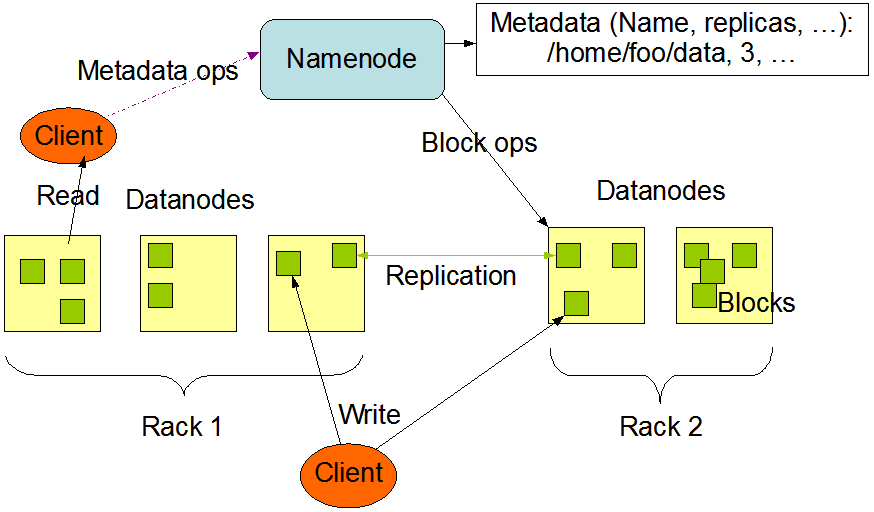
\includegraphics[scale=0.7]{resources/images/Background/hdfs_arch.png}
\label{fig:hadoop_hdfs}
\caption{HDFS architecture}
\end{figure}

\subsubsection{NameNode}
\label{sssec:nn}

Here I will briefly describe the NameNode

\subsubsection{DataNode}
\label{sssec:dn}

Here I will briefly describe the DataNode
